\documentclass[1p]{elsarticle_modified}
%\bibliographystyle{elsarticle-num}

%\usepackage[colorlinks]{hyperref}
%\usepackage{abbrmath_seonhwa} %\Abb, \Ascr, \Acal ,\Abf, \Afrak
\usepackage{amsfonts}
\usepackage{amssymb}
\usepackage{amsmath}
\usepackage{amsthm}
\usepackage{scalefnt}
\usepackage{amsbsy}
\usepackage{kotex}
\usepackage{caption}
\usepackage{subfig}
\usepackage{color}
\usepackage{graphicx}
\usepackage{xcolor} %% white, black, red, green, blue, cyan, magenta, yellow
\usepackage{float}
\usepackage{setspace}
\usepackage{hyperref}

\usepackage{tikz}
\usetikzlibrary{arrows}

\usepackage{multirow}
\usepackage{array} % fixed length table
\usepackage{hhline}

%%%%%%%%%%%%%%%%%%%%%
\makeatletter
\renewcommand*\env@matrix[1][\arraystretch]{%
	\edef\arraystretch{#1}%
	\hskip -\arraycolsep
	\let\@ifnextchar\new@ifnextchar
	\array{*\c@MaxMatrixCols c}}
\makeatother %https://tex.stackexchange.com/questions/14071/how-can-i-increase-the-line-spacing-in-a-matrix
%%%%%%%%%%%%%%%

\usepackage[normalem]{ulem}

\newcommand{\msout}[1]{\ifmmode\text{\sout{\ensuremath{#1}}}\else\sout{#1}\fi}
%SOURCE: \msout is \stkout macro in https://tex.stackexchange.com/questions/20609/strikeout-in-math-mode

\newcommand{\cancel}[1]{
	\ifmmode
	{\color{red}\msout{#1}}
	\else
	{\color{red}\sout{#1}}
	\fi
}

\newcommand{\add}[1]{
	{\color{blue}\uwave{#1}}
}

\newcommand{\replace}[2]{
	\ifmmode
	{\color{red}\msout{#1}}{\color{blue}\uwave{#2}}
	\else
	{\color{red}\sout{#1}}{\color{blue}\uwave{#2}}
	\fi
}

\newcommand{\Sol}{\mathcal{S}} %segment
\newcommand{\D}{D} %diagram
\newcommand{\A}{\mathcal{A}} %arc


%%%%%%%%%%%%%%%%%%%%%%%%%%%%%5 test

\def\sl{\operatorname{\textup{SL}}(2,\Cbb)}
\def\psl{\operatorname{\textup{PSL}}(2,\Cbb)}
\def\quan{\mkern 1mu \triangleright \mkern 1mu}

\theoremstyle{definition}
\newtheorem{thm}{Theorem}[section]
\newtheorem{prop}[thm]{Proposition}
\newtheorem{lem}[thm]{Lemma}
\newtheorem{ques}[thm]{Question}
\newtheorem{cor}[thm]{Corollary}
\newtheorem{defn}[thm]{Definition}
\newtheorem{exam}[thm]{Example}
\newtheorem{rmk}[thm]{Remark}
\newtheorem{alg}[thm]{Algorithm}

\newcommand{\I}{\sqrt{-1}}
\begin{document}

%\begin{frontmatter}
%
%\title{Boundary parabolic representations of knots up to 8 crossings}
%
%%% Group authors per affiliation:
%\author{Yunhi Cho} 
%\address{Department of Mathematics, University of Seoul, Seoul, Korea}
%\ead{yhcho@uos.ac.kr}
%
%
%\author{Seonhwa Kim} %\fnref{s_kim}}
%\address{Center for Geometry and Physics, Institute for Basic Science, Pohang, 37673, Korea}
%\ead{ryeona17@ibs.re.kr}
%
%\author{Hyuk Kim}
%\address{Department of Mathematical Sciences, Seoul National University, Seoul 08826, Korea}
%\ead{hyukkim@snu.ac.kr}
%
%\author{Seokbeom Yoon}
%\address{Department of Mathematical Sciences, Seoul National University, Seoul, 08826,  Korea}
%\ead{sbyoon15@snu.ac.kr}
%
%\begin{abstract}
%We find all boundary parabolic representation of knots up to 8 crossings.
%
%\end{abstract}
%\begin{keyword}
%    \MSC[2010] 57M25 
%\end{keyword}
%
%\end{frontmatter}

%\linenumbers
%\tableofcontents
%
\newcommand\colored[1]{\textcolor{white}{\rule[-0.35ex]{0.8em}{1.4ex}}\kern-0.8em\color{red} #1}%
%\newcommand\colored[1]{\textcolor{white}{ #1}\kern-2.17ex	\textcolor{white}{ #1}\kern-1.81ex	\textcolor{white}{ #1}\kern-2.15ex\color{red}#1	}

{\Large $\underline{12a_{0158}~(K12a_{0158})}$}

\setlength{\tabcolsep}{10pt}
\renewcommand{\arraystretch}{1.6}
\vspace{1cm}\begin{tabular}{m{100pt}>{\centering\arraybackslash}m{274pt}}
\multirow{5}{120pt}{
	\centering
	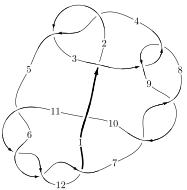
\includegraphics[width=112pt]{../../../GIT/diagram.site/Diagrams/png/959_12a_0158.png}\\
\ \ \ A knot diagram\footnotemark}&
\allowdisplaybreaks
\textbf{Linearized knot diagam} \\
\cline{2-2}
 &
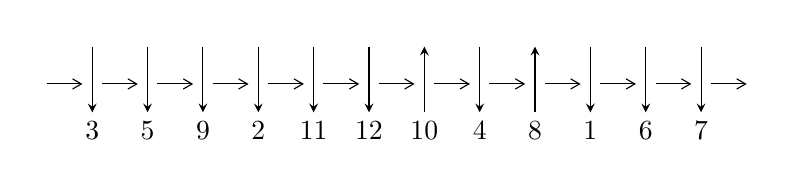
\begin{tikzpicture}[x=20pt, y=17pt]
	% nodes
	\node (C0) at (0, 0) {};
	\node (C1) at (1, 0) {};
	\node (C1U) at (1, +1) {};
	\node (C1D) at (1, -1) {3};

	\node (C2) at (2, 0) {};
	\node (C2U) at (2, +1) {};
	\node (C2D) at (2, -1) {5};

	\node (C3) at (3, 0) {};
	\node (C3U) at (3, +1) {};
	\node (C3D) at (3, -1) {9};

	\node (C4) at (4, 0) {};
	\node (C4U) at (4, +1) {};
	\node (C4D) at (4, -1) {2};

	\node (C5) at (5, 0) {};
	\node (C5U) at (5, +1) {};
	\node (C5D) at (5, -1) {11};

	\node (C6) at (6, 0) {};
	\node (C6U) at (6, +1) {};
	\node (C6D) at (6, -1) {12};

	\node (C7) at (7, 0) {};
	\node (C7U) at (7, +1) {};
	\node (C7D) at (7, -1) {10};

	\node (C8) at (8, 0) {};
	\node (C8U) at (8, +1) {};
	\node (C8D) at (8, -1) {4};

	\node (C9) at (9, 0) {};
	\node (C9U) at (9, +1) {};
	\node (C9D) at (9, -1) {8};

	\node (C10) at (10, 0) {};
	\node (C10U) at (10, +1) {};
	\node (C10D) at (10, -1) {1};

	\node (C11) at (11, 0) {};
	\node (C11U) at (11, +1) {};
	\node (C11D) at (11, -1) {6};

	\node (C12) at (12, 0) {};
	\node (C12U) at (12, +1) {};
	\node (C12D) at (12, -1) {7};
	\node (C13) at (13, 0) {};

	% arrows
	\draw[->,>={angle 60}]
	(C0) edge (C1) (C1) edge (C2) (C2) edge (C3) (C3) edge (C4) (C4) edge (C5) (C5) edge (C6) (C6) edge (C7) (C7) edge (C8) (C8) edge (C9) (C9) edge (C10) (C10) edge (C11) (C11) edge (C12) (C12) edge (C13) ;	\draw[->,>=stealth]
	(C1U) edge (C1D) (C2U) edge (C2D) (C3U) edge (C3D) (C4U) edge (C4D) (C5U) edge (C5D) (C6U) edge (C6D) (C7D) edge (C7U) (C8U) edge (C8D) (C9D) edge (C9U) (C10U) edge (C10D) (C11U) edge (C11D) (C12U) edge (C12D) ;
	\end{tikzpicture} \\
\hhline{~~} \\& 
\textbf{Solving Sequence} \\ \cline{2-2} 
 &
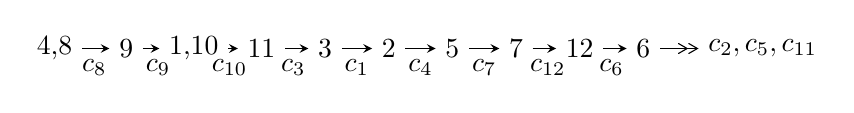
\begin{tikzpicture}[x=23pt, y=7pt]
	% node
	\node (A0) at (-1/8, 0) {4,8};
	\node (A1) at (1, 0) {9};
	\node (A2) at (33/16, 0) {1,10};
	\node (A3) at (25/8, 0) {11};
	\node (A4) at (33/8, 0) {3};
	\node (A5) at (41/8, 0) {2};
	\node (A6) at (49/8, 0) {5};
	\node (A7) at (57/8, 0) {7};
	\node (A8) at (65/8, 0) {12};
	\node (A9) at (73/8, 0) {6};
	\node (C1) at (1/2, -1) {$c_{8}$};
	\node (C2) at (3/2, -1) {$c_{9}$};
	\node (C3) at (21/8, -1) {$c_{10}$};
	\node (C4) at (29/8, -1) {$c_{3}$};
	\node (C5) at (37/8, -1) {$c_{1}$};
	\node (C6) at (45/8, -1) {$c_{4}$};
	\node (C7) at (53/8, -1) {$c_{7}$};
	\node (C8) at (61/8, -1) {$c_{12}$};
	\node (C9) at (69/8, -1) {$c_{6}$};
	\node (A10) at (11, 0) {$c_{2},c_{5},c_{11}$};

	% edge
	\draw[->,>=stealth]	
	(A0) edge (A1) (A1) edge (A2) (A2) edge (A3) (A3) edge (A4) (A4) edge (A5) (A5) edge (A6) (A6) edge (A7) (A7) edge (A8) (A8) edge (A9) ;
	\draw[->>,>={angle 60}]	
	(A9) edge (A10);
\end{tikzpicture} \\ 

\end{tabular} \\

\footnotetext{
The image of knot diagram is generated by the software ``\textbf{Draw programme}" developed by Andrew Bartholomew(\url{http://www.layer8.co.uk/maths/draw/index.htm\#Running-draw}), where we modified some parts for our purpose(\url{https://github.com/CATsTAILs/LinksPainter}).
}\phantom \\ \newline 
\centering \textbf{Ideals for irreducible components\footnotemark of $X_{\text{par}}$} 
 
\begin{align*}
I^u_{1}&=\langle 
-4.37013\times10^{32} u^{60}+1.07931\times10^{33} u^{59}+\cdots+2.13053\times10^{33} b+2.55159\times10^{32},\\
\phantom{I^u_{1}}&\phantom{= \langle  }-1.77317\times10^{32} u^{60}+4.83859\times10^{32} u^{59}+\cdots+1.06527\times10^{33} a+3.22263\times10^{33},\;u^{61}- u^{60}+\cdots+8 u+4\rangle \\
\\
I^v_{1}&=\langle 
a,\;b+v+1,\;v^2+v-1\rangle \\
\end{align*}
\raggedright * 2 irreducible components of $\dim_{\mathbb{C}}=0$, with total 63 representations.\\
\footnotetext{All coefficients of polynomials are rational numbers. But the coefficients are sometimes approximated in decimal forms when there is not enough margin.}
\newpage
\renewcommand{\arraystretch}{1}
\centering \section*{I. $I^u_{1}= \langle -4.37\times10^{32} u^{60}+1.08\times10^{33} u^{59}+\cdots+2.13\times10^{33} b+2.55\times10^{32},\;-1.77\times10^{32} u^{60}+4.84\times10^{32} u^{59}+\cdots+1.07\times10^{33} a+3.22\times10^{33},\;u^{61}- u^{60}+\cdots+8 u+4 \rangle$}
\flushleft \textbf{(i) Arc colorings}\\
\begin{tabular}{m{7pt} m{180pt} m{7pt} m{180pt} }
\flushright $a_{4}=$&$\begin{pmatrix}0\\u\end{pmatrix}$ \\
\flushright $a_{8}=$&$\begin{pmatrix}1\\0\end{pmatrix}$ \\
\flushright $a_{9}=$&$\begin{pmatrix}1\\u^2\end{pmatrix}$ \\
\flushright $a_{1}=$&$\begin{pmatrix}0.166453 u^{60}-0.454214 u^{59}+\cdots-5.04302 u-3.02519\\0.205119 u^{60}-0.506592 u^{59}+\cdots+1.80715 u-0.119763\end{pmatrix}$ \\
\flushright $a_{10}=$&$\begin{pmatrix}u^2+1\\u^2\end{pmatrix}$ \\
\flushright $a_{11}=$&$\begin{pmatrix}-0.0499331 u^{60}-0.0191878 u^{59}+\cdots+4.34689 u+1.61382\\0.531140 u^{60}-0.796906 u^{59}+\cdots+4.86494 u+0.379014\end{pmatrix}$ \\
\flushright $a_{3}=$&$\begin{pmatrix}u\\u^3+u\end{pmatrix}$ \\
\flushright $a_{2}=$&$\begin{pmatrix}0.308153 u^{60}-0.583793 u^{59}+\cdots-4.74082 u-3.17923\\0.351153 u^{60}-0.680255 u^{59}+\cdots+1.44558 u-0.322290\end{pmatrix}$ \\
\flushright $a_{5}=$&$\begin{pmatrix}0.152571 u^{60}-0.191082 u^{59}+\cdots+5.21389 u+1.75438\\0.319024 u^{60}-0.645296 u^{59}+\cdots+0.170875 u-1.27081\end{pmatrix}$ \\
\flushright $a_{7}=$&$\begin{pmatrix}u^4+u^2+1\\u^4\end{pmatrix}$ \\
\flushright $a_{12}=$&$\begin{pmatrix}0.394171 u^{60}-0.666399 u^{59}+\cdots-4.85797 u-3.23772\\0.323761 u^{60}-0.610161 u^{59}+\cdots-0.328448 u-1.25482\end{pmatrix}$ \\
\flushright $a_{6}=$&$\begin{pmatrix}-0.711527 u^{60}+0.890795 u^{59}+\cdots-2.81563 u-0.209751\\-0.127525 u^{60}+0.512045 u^{59}+\cdots-3.76247 u-1.00960\end{pmatrix}$\\&\end{tabular}
\flushleft \textbf{(ii) Obstruction class $= -1$}\\~\\
\flushleft \textbf{(iii) Cusp Shapes $= -1.26579 u^{60}+1.94808 u^{59}+\cdots+11.8662 u-2.65853$}\\~\\
\newpage\renewcommand{\arraystretch}{1}
\flushleft \textbf{(iv) u-Polynomials at the component}\newline \\
\begin{tabular}{m{50pt}|m{274pt}}
Crossings & \hspace{64pt}u-Polynomials at each crossing \\
\hline $$\begin{aligned}c_{1}\end{aligned}$$&$\begin{aligned}
&u^{61}+35 u^{60}+\cdots+40 u+1
\end{aligned}$\\
\hline $$\begin{aligned}c_{2},c_{4}\end{aligned}$$&$\begin{aligned}
&u^{61}-3 u^{60}+\cdots+2 u+1
\end{aligned}$\\
\hline $$\begin{aligned}c_{3},c_{8}\end{aligned}$$&$\begin{aligned}
&u^{61}- u^{60}+\cdots+8 u+4
\end{aligned}$\\
\hline $$\begin{aligned}c_{5},c_{6},c_{11}\\c_{12}\end{aligned}$$&$\begin{aligned}
&u^{61}+2 u^{60}+\cdots+u+1
\end{aligned}$\\
\hline $$\begin{aligned}c_{7},c_{9}\end{aligned}$$&$\begin{aligned}
&u^{61}-15 u^{60}+\cdots-88 u+16
\end{aligned}$\\
\hline $$\begin{aligned}c_{10}\end{aligned}$$&$\begin{aligned}
&u^{61}-20 u^{60}+\cdots-33811 u+6497
\end{aligned}$\\
\hline
\end{tabular}\\~\\
\newpage\renewcommand{\arraystretch}{1}
\flushleft \textbf{(v) Riley Polynomials at the component}\newline \\
\begin{tabular}{m{50pt}|m{274pt}}
Crossings & \hspace{64pt}Riley Polynomials at each crossing \\
\hline $$\begin{aligned}c_{1}\end{aligned}$$&$\begin{aligned}
&y^{61}-15 y^{60}+\cdots+992 y-1
\end{aligned}$\\
\hline $$\begin{aligned}c_{2},c_{4}\end{aligned}$$&$\begin{aligned}
&y^{61}-35 y^{60}+\cdots+40 y-1
\end{aligned}$\\
\hline $$\begin{aligned}c_{3},c_{8}\end{aligned}$$&$\begin{aligned}
&y^{61}+15 y^{60}+\cdots-88 y-16
\end{aligned}$\\
\hline $$\begin{aligned}c_{5},c_{6},c_{11}\\c_{12}\end{aligned}$$&$\begin{aligned}
&y^{61}-72 y^{60}+\cdots+13 y-1
\end{aligned}$\\
\hline $$\begin{aligned}c_{7},c_{9}\end{aligned}$$&$\begin{aligned}
&y^{61}+59 y^{60}+\cdots+9760 y-256
\end{aligned}$\\
\hline $$\begin{aligned}c_{10}\end{aligned}$$&$\begin{aligned}
&y^{61}-36 y^{60}+\cdots-229814295 y-42211009
\end{aligned}$\\
\hline
\end{tabular}\\~\\
\newpage\flushleft \textbf{(vi) Complex Volumes and Cusp Shapes}
$$\begin{array}{c|c|c}  
\text{Solutions to }I^u_{1}& \I (\text{vol} + \sqrt{-1}CS) & \text{Cusp shape}\\
 \hline 
\begin{aligned}
u &= -0.238487 + 0.953197 I \\
a &= -0.003755 + 0.877090 I \\
b &= -0.178706 + 0.107732 I\end{aligned}
 & \phantom{-}2.09116 + 2.27253 I & -4.25062 - 5.15678 I \\ \hline\begin{aligned}
u &= -0.238487 - 0.953197 I \\
a &= -0.003755 - 0.877090 I \\
b &= -0.178706 - 0.107732 I\end{aligned}
 & \phantom{-}2.09116 - 2.27253 I & -4.25062 + 5.15678 I \\ \hline\begin{aligned}
u &= -0.307970 + 0.970251 I \\
a &= \phantom{-}0.0336117 - 0.1292320 I \\
b &= \phantom{-}0.942071 + 0.219289 I\end{aligned}
 & \phantom{-}1.65969 + 3.31321 I & -4.58003 - 3.95738 I \\ \hline\begin{aligned}
u &= -0.307970 - 0.970251 I \\
a &= \phantom{-}0.0336117 + 0.1292320 I \\
b &= \phantom{-}0.942071 - 0.219289 I\end{aligned}
 & \phantom{-}1.65969 - 3.31321 I & -4.58003 + 3.95738 I \\ \hline\begin{aligned}
u &= -0.877601 + 0.378203 I \\
a &= \phantom{-}0.207288 - 0.357685 I \\
b &= \phantom{-}0.447467 + 0.371493 I\end{aligned}
 & -9.07110 - 3.90521 I & -14.6512 + 4.5873 I \\ \hline\begin{aligned}
u &= -0.877601 - 0.378203 I \\
a &= \phantom{-}0.207288 + 0.357685 I \\
b &= \phantom{-}0.447467 - 0.371493 I\end{aligned}
 & -9.07110 + 3.90521 I & -14.6512 - 4.5873 I \\ \hline\begin{aligned}
u &= \phantom{-}0.084785 + 0.946752 I \\
a &= -0.080363 + 0.669261 I \\
b &= \phantom{-}0.531909 + 0.161258 I\end{aligned}
 & \phantom{-}2.57667 + 0.91135 I & -2.15381 - 4.08068 I \\ \hline\begin{aligned}
u &= \phantom{-}0.084785 - 0.946752 I \\
a &= -0.080363 - 0.669261 I \\
b &= \phantom{-}0.531909 - 0.161258 I\end{aligned}
 & \phantom{-}2.57667 - 0.91135 I & -2.15381 + 4.08068 I \\ \hline\begin{aligned}
u &= \phantom{-}0.077209 + 1.056450 I \\
a &= \phantom{-}0.297681 + 0.382384 I \\
b &= -0.928442 + 0.127233 I\end{aligned}
 & -3.28717 - 2.31394 I & -7.12059 + 3.62918 I \\ \hline\begin{aligned}
u &= \phantom{-}0.077209 - 1.056450 I \\
a &= \phantom{-}0.297681 - 0.382384 I \\
b &= -0.928442 - 0.127233 I\end{aligned}
 & -3.28717 + 2.31394 I & -7.12059 - 3.62918 I\\
 \hline 
 \end{array}$$\newpage$$\begin{array}{c|c|c}  
\text{Solutions to }I^u_{1}& \I (\text{vol} + \sqrt{-1}CS) & \text{Cusp shape}\\
 \hline 
\begin{aligned}
u &= \phantom{-}0.359746 + 1.016880 I \\
a &= \phantom{-}0.062599 + 1.101460 I \\
b &= -0.217088 + 0.019866 I\end{aligned}
 & -4.85916 - 4.06193 I & -8.00000 + 3.62400 I \\ \hline\begin{aligned}
u &= \phantom{-}0.359746 - 1.016880 I \\
a &= \phantom{-}0.062599 - 1.101460 I \\
b &= -0.217088 - 0.019866 I\end{aligned}
 & -4.85916 + 4.06193 I & -8.00000 - 3.62400 I \\ \hline\begin{aligned}
u &= \phantom{-}0.410008 + 1.014890 I \\
a &= -0.012002 - 0.459759 I \\
b &= -0.721661 + 0.144626 I\end{aligned}
 & \phantom{-}0.62509 - 6.72372 I & -8.00000 + 10.31873 I \\ \hline\begin{aligned}
u &= \phantom{-}0.410008 - 1.014890 I \\
a &= -0.012002 + 0.459759 I \\
b &= -0.721661 - 0.144626 I\end{aligned}
 & \phantom{-}0.62509 + 6.72372 I & -8.00000 - 10.31873 I \\ \hline\begin{aligned}
u &= \phantom{-}0.808032 + 0.816831 I \\
a &= \phantom{-}1.00805 + 1.02708 I \\
b &= \phantom{-}0.03711 + 1.94913 I\end{aligned}
 & -4.47605 + 0.47564 I & \phantom{-0.000000 } 0 \\ \hline\begin{aligned}
u &= \phantom{-}0.808032 - 0.816831 I \\
a &= \phantom{-}1.00805 - 1.02708 I \\
b &= \phantom{-}0.03711 - 1.94913 I\end{aligned}
 & -4.47605 - 0.47564 I & \phantom{-0.000000 } 0 \\ \hline\begin{aligned}
u &= -0.749510 + 0.886201 I \\
a &= -0.87056 + 1.16887 I \\
b &= \phantom{-}0.43430 + 1.70385 I\end{aligned}
 & -1.90394 + 2.84541 I & \phantom{-0.000000 } 0 \\ \hline\begin{aligned}
u &= -0.749510 - 0.886201 I \\
a &= -0.87056 - 1.16887 I \\
b &= \phantom{-}0.43430 - 1.70385 I\end{aligned}
 & -1.90394 - 2.84541 I & \phantom{-0.000000 } 0 \\ \hline\begin{aligned}
u &= -0.316577 + 0.775281 I \\
a &= \phantom{-}0.34310 - 2.42404 I \\
b &= -0.749506 + 0.387164 I\end{aligned}
 & -9.89951 + 1.70824 I & -13.49720 - 3.89995 I \\ \hline\begin{aligned}
u &= -0.316577 - 0.775281 I \\
a &= \phantom{-}0.34310 + 2.42404 I \\
b &= -0.749506 - 0.387164 I\end{aligned}
 & -9.89951 - 1.70824 I & -13.49720 + 3.89995 I\\
 \hline 
 \end{array}$$\newpage$$\begin{array}{c|c|c}  
\text{Solutions to }I^u_{1}& \I (\text{vol} + \sqrt{-1}CS) & \text{Cusp shape}\\
 \hline 
\begin{aligned}
u &= -0.489410 + 1.059940 I \\
a &= -0.038865 - 0.755001 I \\
b &= \phantom{-}0.369249 + 0.129881 I\end{aligned}
 & -6.69274 + 8.82294 I & \phantom{-0.000000 } 0 \\ \hline\begin{aligned}
u &= -0.489410 - 1.059940 I \\
a &= -0.038865 + 0.755001 I \\
b &= \phantom{-}0.369249 - 0.129881 I\end{aligned}
 & -6.69274 - 8.82294 I & \phantom{-0.000000 } 0 \\ \hline\begin{aligned}
u &= \phantom{-}0.849526 + 0.813861 I \\
a &= -1.44747 - 1.16596 I \\
b &= -0.11881 - 1.83683 I\end{aligned}
 & -5.74001 + 1.43814 I & \phantom{-0.000000 } 0 \\ \hline\begin{aligned}
u &= \phantom{-}0.849526 - 0.813861 I \\
a &= -1.44747 + 1.16596 I \\
b &= -0.11881 + 1.83683 I\end{aligned}
 & -5.74001 - 1.43814 I & \phantom{-0.000000 } 0 \\ \hline\begin{aligned}
u &= \phantom{-}0.757519 + 0.305031 I \\
a &= \phantom{-}0.149859 - 0.548164 I \\
b &= -0.040871 + 0.285650 I\end{aligned}
 & -1.78875 + 2.52359 I & -12.4907 - 7.4949 I \\ \hline\begin{aligned}
u &= \phantom{-}0.757519 - 0.305031 I \\
a &= \phantom{-}0.149859 + 0.548164 I \\
b &= -0.040871 - 0.285650 I\end{aligned}
 & -1.78875 - 2.52359 I & -12.4907 + 7.4949 I \\ \hline\begin{aligned}
u &= -0.874218 + 0.804569 I \\
a &= -1.15410 + 0.99565 I \\
b &= -0.28100 + 2.30195 I\end{aligned}
 & -12.87930 - 2.42278 I & \phantom{-0.000000 } 0 \\ \hline\begin{aligned}
u &= -0.874218 - 0.804569 I \\
a &= -1.15410 - 0.99565 I \\
b &= -0.28100 - 2.30195 I\end{aligned}
 & -12.87930 + 2.42278 I & \phantom{-0.000000 } 0 \\ \hline\begin{aligned}
u &= -0.821847 + 0.871851 I \\
a &= \phantom{-}1.56651 - 1.37568 I \\
b &= -0.35452 - 2.07289 I\end{aligned}
 & -8.17948 + 2.03351 I & \phantom{-0.000000 } 0 \\ \hline\begin{aligned}
u &= -0.821847 - 0.871851 I \\
a &= \phantom{-}1.56651 + 1.37568 I \\
b &= -0.35452 + 2.07289 I\end{aligned}
 & -8.17948 - 2.03351 I & \phantom{-0.000000 } 0\\
 \hline 
 \end{array}$$\newpage$$\begin{array}{c|c|c}  
\text{Solutions to }I^u_{1}& \I (\text{vol} + \sqrt{-1}CS) & \text{Cusp shape}\\
 \hline 
\begin{aligned}
u &= \phantom{-}0.241710 + 0.747099 I \\
a &= -0.465874 + 0.305697 I \\
b &= -1.270210 + 0.529709 I\end{aligned}
 & -1.94835 - 1.41549 I & -11.33185 + 4.43113 I \\ \hline\begin{aligned}
u &= \phantom{-}0.241710 - 0.747099 I \\
a &= -0.465874 - 0.305697 I \\
b &= -1.270210 - 0.529709 I\end{aligned}
 & -1.94835 + 1.41549 I & -11.33185 - 4.43113 I \\ \hline\begin{aligned}
u &= \phantom{-}0.772724 + 0.137846 I \\
a &= \phantom{-}0.672930 + 0.110054 I \\
b &= \phantom{-}0.895434 - 0.127416 I\end{aligned}
 & -7.72551 + 0.23364 I & -12.50787 + 1.31729 I \\ \hline\begin{aligned}
u &= \phantom{-}0.772724 - 0.137846 I \\
a &= \phantom{-}0.672930 - 0.110054 I \\
b &= \phantom{-}0.895434 + 0.127416 I\end{aligned}
 & -7.72551 - 0.23364 I & -12.50787 - 1.31729 I \\ \hline\begin{aligned}
u &= -0.909481 + 0.809234 I \\
a &= \phantom{-}1.55609 - 0.96630 I \\
b &= \phantom{-}0.57813 - 2.04844 I\end{aligned}
 & -8.07107 - 4.97454 I & \phantom{-0.000000 } 0 \\ \hline\begin{aligned}
u &= -0.909481 - 0.809234 I \\
a &= \phantom{-}1.55609 + 0.96630 I \\
b &= \phantom{-}0.57813 + 2.04844 I\end{aligned}
 & -8.07107 + 4.97454 I & \phantom{-0.000000 } 0 \\ \hline\begin{aligned}
u &= \phantom{-}0.836848 + 0.884467 I \\
a &= -1.10413 - 1.59303 I \\
b &= -0.05000 - 2.92120 I\end{aligned}
 & -16.6735 - 2.0703 I & \phantom{-0.000000 } 0 \\ \hline\begin{aligned}
u &= \phantom{-}0.836848 - 0.884467 I \\
a &= -1.10413 + 1.59303 I \\
b &= -0.05000 + 2.92120 I\end{aligned}
 & -16.6735 + 2.0703 I & \phantom{-0.000000 } 0 \\ \hline\begin{aligned}
u &= -0.805476 + 0.918966 I \\
a &= \phantom{-}0.92783 - 1.56312 I \\
b &= -0.19783 - 2.45697 I\end{aligned}
 & -8.03154 + 4.05119 I & \phantom{-0.000000 } 0 \\ \hline\begin{aligned}
u &= -0.805476 - 0.918966 I \\
a &= \phantom{-}0.92783 + 1.56312 I \\
b &= -0.19783 + 2.45697 I\end{aligned}
 & -8.03154 - 4.05119 I & \phantom{-0.000000 } 0\\
 \hline 
 \end{array}$$\newpage$$\begin{array}{c|c|c}  
\text{Solutions to }I^u_{1}& \I (\text{vol} + \sqrt{-1}CS) & \text{Cusp shape}\\
 \hline 
\begin{aligned}
u &= \phantom{-}0.776141 + 0.950673 I \\
a &= \phantom{-}0.90967 + 1.32399 I \\
b &= -0.83918 + 1.88849 I\end{aligned}
 & -4.06730 - 6.42529 I & \phantom{-0.000000 } 0 \\ \hline\begin{aligned}
u &= \phantom{-}0.776141 - 0.950673 I \\
a &= \phantom{-}0.90967 - 1.32399 I \\
b &= -0.83918 - 1.88849 I\end{aligned}
 & -4.06730 + 6.42529 I & \phantom{-0.000000 } 0 \\ \hline\begin{aligned}
u &= \phantom{-}0.824923 + 0.918769 I \\
a &= -1.71708 - 1.47330 I \\
b &= \phantom{-}0.63383 - 2.39142 I\end{aligned}
 & -16.5663 - 4.1225 I & \phantom{-0.000000 } 0 \\ \hline\begin{aligned}
u &= \phantom{-}0.824923 - 0.918769 I \\
a &= -1.71708 + 1.47330 I \\
b &= \phantom{-}0.63383 + 2.39142 I\end{aligned}
 & -16.5663 + 4.1225 I & \phantom{-0.000000 } 0 \\ \hline\begin{aligned}
u &= \phantom{-}0.797214 + 0.969907 I \\
a &= -0.74216 - 1.63736 I \\
b &= \phantom{-}0.66652 - 2.12988 I\end{aligned}
 & -5.25621 - 7.57674 I & \phantom{-0.000000 } 0 \\ \hline\begin{aligned}
u &= \phantom{-}0.797214 - 0.969907 I \\
a &= -0.74216 + 1.63736 I \\
b &= \phantom{-}0.66652 + 2.12988 I\end{aligned}
 & -5.25621 + 7.57674 I & \phantom{-0.000000 } 0 \\ \hline\begin{aligned}
u &= \phantom{-}0.949600 + 0.823547 I \\
a &= -1.68518 - 0.86336 I \\
b &= -0.86700 - 2.32515 I\end{aligned}
 & -16.4115 + 7.1396 I & \phantom{-0.000000 } 0 \\ \hline\begin{aligned}
u &= \phantom{-}0.949600 - 0.823547 I \\
a &= -1.68518 + 0.86336 I \\
b &= -0.86700 + 2.32515 I\end{aligned}
 & -16.4115 - 7.1396 I & \phantom{-0.000000 } 0 \\ \hline\begin{aligned}
u &= -0.806362 + 0.985930 I \\
a &= -0.96958 + 1.42164 I \\
b &= \phantom{-}1.10553 + 2.10803 I\end{aligned}
 & -12.3142 + 8.6618 I & \phantom{-0.000000 } 0 \\ \hline\begin{aligned}
u &= -0.806362 - 0.985930 I \\
a &= -0.96958 - 1.42164 I \\
b &= \phantom{-}1.10553 - 2.10803 I\end{aligned}
 & -12.3142 - 8.6618 I & \phantom{-0.000000 } 0\\
 \hline 
 \end{array}$$\newpage$$\begin{array}{c|c|c}  
\text{Solutions to }I^u_{1}& \I (\text{vol} + \sqrt{-1}CS) & \text{Cusp shape}\\
 \hline 
\begin{aligned}
u &= -0.823074 + 1.001050 I \\
a &= \phantom{-}0.68683 - 1.78798 I \\
b &= -1.13111 - 2.20407 I\end{aligned}
 & -7.46084 + 11.37220 I & \phantom{-0.000000 } 0 \\ \hline\begin{aligned}
u &= -0.823074 - 1.001050 I \\
a &= \phantom{-}0.68683 + 1.78798 I \\
b &= -1.13111 + 2.20407 I\end{aligned}
 & -7.46084 - 11.37220 I & \phantom{-0.000000 } 0 \\ \hline\begin{aligned}
u &= \phantom{-}0.848261 + 1.018330 I \\
a &= -0.67747 - 1.91157 I \\
b &= \phantom{-}1.48348 - 2.35344 I\end{aligned}
 & -15.7786 - 13.7453 I & \phantom{-0.000000 } 0 \\ \hline\begin{aligned}
u &= \phantom{-}0.848261 - 1.018330 I \\
a &= -0.67747 + 1.91157 I \\
b &= \phantom{-}1.48348 + 2.35344 I\end{aligned}
 & -15.7786 + 13.7453 I & \phantom{-0.000000 } 0 \\ \hline\begin{aligned}
u &= -0.308299 + 0.596152 I \\
a &= \phantom{-}0.945489 + 0.457470 I \\
b &= \phantom{-}2.00842 + 0.79172 I\end{aligned}
 & -10.52170 + 0.86189 I & -12.7781 - 7.9081 I \\ \hline\begin{aligned}
u &= -0.308299 - 0.596152 I \\
a &= \phantom{-}0.945489 - 0.457470 I \\
b &= \phantom{-}2.00842 - 0.79172 I\end{aligned}
 & -10.52170 - 0.86189 I & -12.7781 + 7.9081 I \\ \hline\begin{aligned}
u &= \phantom{-}0.254491 + 0.574517 I \\
a &= \phantom{-}0.11821 - 2.36867 I \\
b &= \phantom{-}0.311978 + 0.275962 I\end{aligned}
 & -2.54655 - 0.75490 I & -10.56290 + 9.15741 I \\ \hline\begin{aligned}
u &= \phantom{-}0.254491 - 0.574517 I \\
a &= \phantom{-}0.11821 + 2.36867 I \\
b &= \phantom{-}0.311978 - 0.275962 I\end{aligned}
 & -2.54655 + 0.75490 I & -10.56290 - 9.15741 I \\ \hline\begin{aligned}
u &= -0.612829 + 0.106029 I \\
a &= -0.809358 - 0.377022 I \\
b &= -0.294046 + 0.149479 I\end{aligned}
 & -1.002850 - 0.150257 I & -9.43253 - 1.75186 I \\ \hline\begin{aligned}
u &= -0.612829 - 0.106029 I \\
a &= -0.809358 + 0.377022 I \\
b &= -0.294046 - 0.149479 I\end{aligned}
 & -1.002850 + 0.150257 I & -9.43253 + 1.75186 I\\
 \hline 
 \end{array}$$\newpage$$\begin{array}{c|c|c}  
\text{Solutions to }I^u_{1}& \I (\text{vol} + \sqrt{-1}CS) & \text{Cusp shape}\\
 \hline 
\begin{aligned}
u &= -0.415187\phantom{ +0.000000I} \\
a &= -0.415618\phantom{ +0.000000I} \\
b &= -0.410931\phantom{ +0.000000I}\end{aligned}
 & -0.737929\phantom{ +0.000000I} & -13.3140\phantom{ +0.000000I}\\
 \hline 
 \end{array}$$\newpage\newpage\renewcommand{\arraystretch}{1}
\centering \section*{II. $I^v_{1}= \langle a,\;b+v+1,\;v^2+v-1 \rangle$}
\flushleft \textbf{(i) Arc colorings}\\
\begin{tabular}{m{7pt} m{180pt} m{7pt} m{180pt} }
\flushright $a_{4}=$&$\begin{pmatrix}v\\0\end{pmatrix}$ \\
\flushright $a_{8}=$&$\begin{pmatrix}1\\0\end{pmatrix}$ \\
\flushright $a_{9}=$&$\begin{pmatrix}1\\0\end{pmatrix}$ \\
\flushright $a_{1}=$&$\begin{pmatrix}0\\- v-1\end{pmatrix}$ \\
\flushright $a_{10}=$&$\begin{pmatrix}1\\0\end{pmatrix}$ \\
\flushright $a_{11}=$&$\begin{pmatrix}1\\v+2\end{pmatrix}$ \\
\flushright $a_{3}=$&$\begin{pmatrix}v\\0\end{pmatrix}$ \\
\flushright $a_{2}=$&$\begin{pmatrix}v\\- v-1\end{pmatrix}$ \\
\flushright $a_{5}=$&$\begin{pmatrix}0\\v+1\end{pmatrix}$ \\
\flushright $a_{7}=$&$\begin{pmatrix}1\\0\end{pmatrix}$ \\
\flushright $a_{12}=$&$\begin{pmatrix}- v-1\\- v-1\end{pmatrix}$ \\
\flushright $a_{6}=$&$\begin{pmatrix}- v-1\\- v-2\end{pmatrix}$\\&\end{tabular}
\flushleft \textbf{(ii) Obstruction class $= 1$}\\~\\
\flushleft \textbf{(iii) Cusp Shapes $= -15$}\\~\\
\newpage\renewcommand{\arraystretch}{1}
\flushleft \textbf{(iv) u-Polynomials at the component}\newline \\
\begin{tabular}{m{50pt}|m{274pt}}
Crossings & \hspace{64pt}u-Polynomials at each crossing \\
\hline $$\begin{aligned}c_{1},c_{2}\end{aligned}$$&$\begin{aligned}
&(u-1)^2
\end{aligned}$\\
\hline $$\begin{aligned}c_{3},c_{7},c_{8}\\c_{9}\end{aligned}$$&$\begin{aligned}
&u^2
\end{aligned}$\\
\hline $$\begin{aligned}c_{4}\end{aligned}$$&$\begin{aligned}
&(u+1)^2
\end{aligned}$\\
\hline $$\begin{aligned}c_{5},c_{6},c_{10}\end{aligned}$$&$\begin{aligned}
&u^2+u-1
\end{aligned}$\\
\hline $$\begin{aligned}c_{11},c_{12}\end{aligned}$$&$\begin{aligned}
&u^2- u-1
\end{aligned}$\\
\hline
\end{tabular}\\~\\
\newpage\renewcommand{\arraystretch}{1}
\flushleft \textbf{(v) Riley Polynomials at the component}\newline \\
\begin{tabular}{m{50pt}|m{274pt}}
Crossings & \hspace{64pt}Riley Polynomials at each crossing \\
\hline $$\begin{aligned}c_{1},c_{2},c_{4}\end{aligned}$$&$\begin{aligned}
&(y-1)^2
\end{aligned}$\\
\hline $$\begin{aligned}c_{3},c_{7},c_{8}\\c_{9}\end{aligned}$$&$\begin{aligned}
&y^2
\end{aligned}$\\
\hline $$\begin{aligned}c_{5},c_{6},c_{10}\\c_{11},c_{12}\end{aligned}$$&$\begin{aligned}
&y^2-3 y+1
\end{aligned}$\\
\hline
\end{tabular}\\~\\
\newpage\flushleft \textbf{(vi) Complex Volumes and Cusp Shapes}
$$\begin{array}{c|c|c}  
\text{Solutions to }I^v_{1}& \I (\text{vol} + \sqrt{-1}CS) & \text{Cusp shape}\\
 \hline 
\begin{aligned}
v &= \phantom{-}0.618034\phantom{ +0.000000I} \\
a &= \phantom{-0.000000 } 0 \\
b &= -1.61803\phantom{ +0.000000I}\end{aligned}
 & -10.5276\phantom{ +0.000000I} & -15.0000\phantom{ +0.000000I} \\ \hline\begin{aligned}
v &= -1.61803\phantom{ +0.000000I} \\
a &= \phantom{-0.000000 } 0 \\
b &= \phantom{-}0.618034\phantom{ +0.000000I}\end{aligned}
 & -2.63189\phantom{ +0.000000I} & -15.0000\phantom{ +0.000000I}\\
 \hline 
 \end{array}$$\newpage
\newpage\renewcommand{\arraystretch}{1}
\centering \section*{ III. u-Polynomials}
\begin{tabular}{m{50pt}|m{274pt}}
Crossings & \hspace{64pt}u-Polynomials at each crossing \\
\hline $$\begin{aligned}c_{1}\end{aligned}$$&$\begin{aligned}
&((u-1)^2)(u^{61}+35 u^{60}+\cdots+40 u+1)
\end{aligned}$\\
\hline $$\begin{aligned}c_{2}\end{aligned}$$&$\begin{aligned}
&((u-1)^2)(u^{61}-3 u^{60}+\cdots+2 u+1)
\end{aligned}$\\
\hline $$\begin{aligned}c_{3},c_{8}\end{aligned}$$&$\begin{aligned}
&u^2(u^{61}- u^{60}+\cdots+8 u+4)
\end{aligned}$\\
\hline $$\begin{aligned}c_{4}\end{aligned}$$&$\begin{aligned}
&((u+1)^2)(u^{61}-3 u^{60}+\cdots+2 u+1)
\end{aligned}$\\
\hline $$\begin{aligned}c_{5},c_{6}\end{aligned}$$&$\begin{aligned}
&(u^2+u-1)(u^{61}+2 u^{60}+\cdots+u+1)
\end{aligned}$\\
\hline $$\begin{aligned}c_{7},c_{9}\end{aligned}$$&$\begin{aligned}
&u^2(u^{61}-15 u^{60}+\cdots-88 u+16)
\end{aligned}$\\
\hline $$\begin{aligned}c_{10}\end{aligned}$$&$\begin{aligned}
&(u^2+u-1)(u^{61}-20 u^{60}+\cdots-33811 u+6497)
\end{aligned}$\\
\hline $$\begin{aligned}c_{11},c_{12}\end{aligned}$$&$\begin{aligned}
&(u^2- u-1)(u^{61}+2 u^{60}+\cdots+u+1)
\end{aligned}$\\
\hline
\end{tabular}\newpage\renewcommand{\arraystretch}{1}
\centering \section*{ IV. Riley Polynomials}
\begin{tabular}{m{50pt}|m{274pt}}
Crossings & \hspace{64pt}Riley Polynomials at each crossing \\
\hline $$\begin{aligned}c_{1}\end{aligned}$$&$\begin{aligned}
&((y-1)^2)(y^{61}-15 y^{60}+\cdots+992 y-1)
\end{aligned}$\\
\hline $$\begin{aligned}c_{2},c_{4}\end{aligned}$$&$\begin{aligned}
&((y-1)^2)(y^{61}-35 y^{60}+\cdots+40 y-1)
\end{aligned}$\\
\hline $$\begin{aligned}c_{3},c_{8}\end{aligned}$$&$\begin{aligned}
&y^2(y^{61}+15 y^{60}+\cdots-88 y-16)
\end{aligned}$\\
\hline $$\begin{aligned}c_{5},c_{6},c_{11}\\c_{12}\end{aligned}$$&$\begin{aligned}
&(y^2-3 y+1)(y^{61}-72 y^{60}+\cdots+13 y-1)
\end{aligned}$\\
\hline $$\begin{aligned}c_{7},c_{9}\end{aligned}$$&$\begin{aligned}
&y^2(y^{61}+59 y^{60}+\cdots+9760 y-256)
\end{aligned}$\\
\hline $$\begin{aligned}c_{10}\end{aligned}$$&$\begin{aligned}
&(y^2-3 y+1)(y^{61}-36 y^{60}+\cdots-2.29814\times10^{8} y-4.22110\times10^{7})
\end{aligned}$\\
\hline
\end{tabular}
\vskip 2pc
\end{document}